\subsubsection{Thành phần chính: Client – Server – Cơ sở dữ liệu}
\indent Hệ thống được thiết kế theo mô hình \textit{client–server} ba lớp, trong đó mỗi thành phần đảm nhận vai trò riêng nhằm bảo đảm hiệu năng và tính bảo mật trong quá trình truyền tải thông tin.

\indent \textbf{Lớp Client:} Ứng dụng được phát triển bằng \textit{Flutter} (ngôn ngữ Dart \cite{dart_spec}), chịu trách nhiệm hiển thị giao diện trò chuyện, quản lý danh sách hội thoại, gửi và nhận tin nhắn.  
Tại lớp này, mọi hoạt động mã hóa và giải mã tin nhắn đều được xử lý hoàn toàn cục bộ nhằm đảm bảo nguyên tắc mã hóa đầu cuối (E2EE), qua đó ngăn máy chủ hoặc tin tặc truy cập trực tiếp vào nội dung tin nhắn.

\indent Ngoài các yêu cầu API thông thường, client duy trì kết nối \textit{WebSocket} ổn định với máy chủ để truyền dữ liệu theo thời gian thực. Khi người dùng tham gia vào một cuộc trò chuyện cụ thể, client sẽ đăng ký vào một phòng tương ứng với mã định danh của cuộc trò chuyện.  
Mọi phiên client khác cùng tham gia hội thoại đó sẽ nhận được sự kiện như tin nhắn mới.

\indent \textbf{Lớp Server:} Máy chủ được triển khai bằng \textit{Node.js} \cite{nodejs_website}, cung cấp \textit{REST API} và \textit{WebSocket Gateway}, đảm nhận vai trò trung gian trong việc truyền tải dữ liệu giữa các người dùng, lưu trữ thông tin và các yêu cầu nghiệp vụ.  
Khi một tin nhắn mới được ghi nhận trong cơ sở dữ liệu, server thực hiện broadcast đến các client đang đăng ký cùng mã định danh của phòng chat, đảm bảo chỉ các thành viên hợp lệ của hội thoại đó mới nhận được dữ liệu.  
Trong toàn bộ quy trình, máy chủ không thực hiện giải mã nội dung tin nhắn mà chỉ lưu trữ bản mã và khóa AES đã được mã hóa bằng khóa công khai RSA, bảo đảm nguyên tắc mã hóa đầu cuối (E2EE).

\indent \textbf{Lớp Cơ sở dữ liệu:} Hệ thống cơ sở dữ liệu được quản lý bằng \textit{MongoDB}, nơi lưu trữ các thực thể chính như người dùng, quan hệ bạn bè, hội thoại, tin nhắn và khóa mã hóa.  
Việc kết hợp \textit{MongoDB Change Streams} cho phép server lắng nghe các thay đổi dữ liệu và chuyển tiếp chúng qua WebSocket. Điều này giúp đảm bảo mọi hành động như gửi tin nhắn hay lời mời kết bạn được thể hiện tức thời trên toàn bộ thiết bị của người dùng.

\indent Hình ~\ref{fig:pic7} minh họa kiến trúc tổng thể của hệ thống, trong đó client chịu trách nhiệm giao tiếp với người dùng, server xử lý nghiệp vụ và điều phối dữ liệu, còn cơ sở dữ liệu đảm bảo tính toàn vẹn và bảo mật thông tin.

\begin{figure}[H]
  \centering
  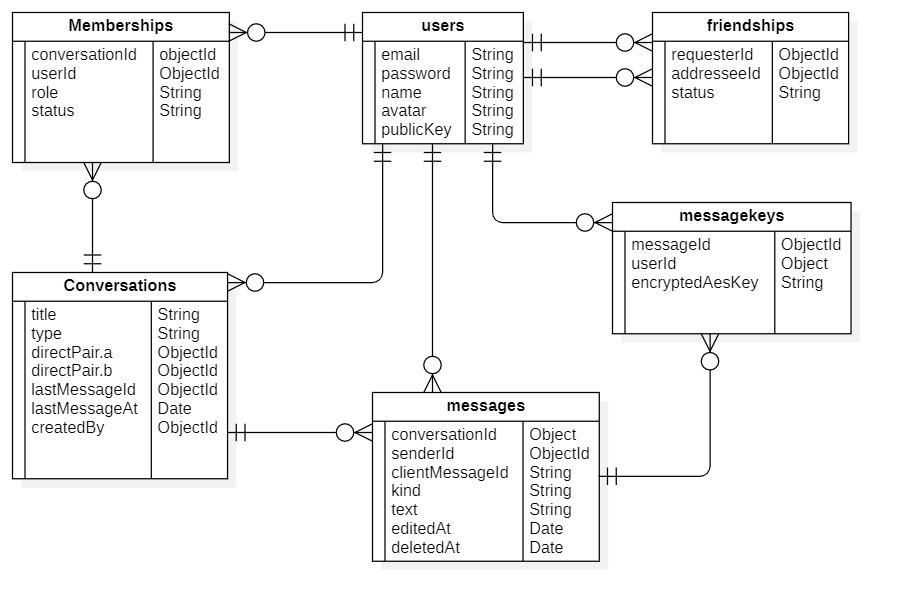
\includegraphics[width=0.95\textwidth]{figures/pic7.png}
  \caption{Mô hình cơ sở dữ liệu của hệ thống.}
  \label{fig:pic7}
\end{figure}


% Bảng conversation
\indent Bảng ~\ref{tab:conversation} mô tả chi tiết các trường dữ liệu của \textbf{bảng Conversation}, được sử dụng để lưu trữ thông tin về các cuộc trò chuyện trong hệ thống.  
Mỗi bản ghi trong bảng biểu thị một cuộc hội thoại, có thể là trò chuyện trực tiếp giữa hai người dùng hoặc trò chuyện nhóm có nhiều thành viên tham gia.

\begin{table}[H]
\centering
\caption{Cấu trúc bảng dữ liệu Conversation.}
\label{tab:conversation}
\begin{tabularx}{\textwidth}{|p{4cm}|p{3cm}|X|}
\hline
\textbf{Trường} & \textbf{Kiểu dữ liệu} & \textbf{Mô tả} \\ \hline
\texttt{type} & String & Loại cuộc trò chuyện: `'direct'` hoặc `'group'`. \\ \hline
\texttt{title} & String & Tên nhóm (chỉ dùng khi là cuộc trò chuyện nhóm). \\ \hline
\texttt{createdBy} & ObjectId (User) & Người tạo cuộc trò chuyện. \\ \hline
\texttt{directPair.a} & ObjectId (User) & Người dùng A trong cuộc trò chuyện. \\ \hline
\texttt{directPair.b} & ObjectId (User) & Người dùng B trong cuộc trò chuyện. \\ \hline
\texttt{lastMessageId} & ObjectId (Message) & Tham chiếu đến tin nhắn gần nhất trong cuộc trò chuyện. \\ \hline
\texttt{lastMessageAt} & Date & Thời gian gửi tin nhắn cuối cùng. \\ \hline
\end{tabularx}
\end{table}


% Bảng friendship
\indent Bảng ~\ref{tab:friendship} mô tả \textbf{cấu trúc bảng dữ liệu Friendship}, được dùng để quản lý mối quan hệ bạn bè giữa các người dùng trong hệ thống.  
Mỗi bản ghi thể hiện một yêu cầu kết bạn cùng với trạng thái hiện tại của mối quan hệ.

\begin{table}[H]
\centering
\caption{Cấu trúc bảng dữ liệu Friendship.}
\label{tab:friendship}
\begin{tabularx}{\textwidth}{|p{3cm}|p{3cm}|X|}
\hline
\textbf{Trường} & \textbf{Kiểu dữ liệu} & \textbf{Mô tả} \\ \hline
\texttt{requesterId} & ObjectId (User) & Người gửi lời mời kết bạn. \\ \hline
\texttt{addresseeId} & ObjectId (User) & Người nhận lời mời kết bạn. \\ \hline
\texttt{status} & String & Trạng thái mối quan hệ: `'pending'`, `'accepted'`, `'blocked'`. \\ \hline
\end{tabularx}
\end{table}

% Bảng membership
\indent Bảng ~\ref{tab:membership} mô tả \textbf{cấu trúc bảng dữ liệu Membership}, được sử dụng để quản lý thông tin thành viên trong mỗi cuộc trò chuyện.  
Mỗi bản ghi thể hiện một người dùng tham gia vào một cuộc hội thoại cùng với vai trò, trạng thái và thời điểm tương tác gần nhất.

\begin{table}[H]
\centering
\caption{Cấu trúc bảng dữ liệu Membership.}
\label{tab:membership}
\begin{tabularx}{\textwidth}{|p{4cm}|p{3cm}|X|}
\hline
\textbf{Trường} & \textbf{Kiểu dữ liệu} & \textbf{Mô tả} \\ \hline
\texttt{conversationId} & ObjectId (Conversation) & Cuộc trò chuyện mà người dùng tham gia. \\ \hline
\texttt{userId} & ObjectId (User) & Người dùng tham gia cuộc trò chuyện. \\ \hline
\texttt{role} & String & Vai trò trong nhóm: `'owner'`, `'admin'`, `'member'`. \\ \hline
\texttt{status} & String & Trạng thái tham gia: `'active'`, `'left'`, `'removed'`. \\ \hline
\end{tabularx}
\end{table}

% Bảng message
\indent Bảng ~\ref{tab:message} trình bày \textbf{cấu trúc bảng dữ liệu Message}, nơi lưu trữ toàn bộ thông tin liên quan đến các tin nhắn trong cuộc trò chuyện.  
Mỗi bản ghi biểu thị một tin nhắn được gửi bởi người dùng, bao gồm nội dung văn bản và các mốc thời gian tương ứng.

\begin{table}[H]
\centering
\caption{Cấu trúc bảng dữ liệu Message.}
\label{tab:message}
\begin{tabularx}{\textwidth}{|p{4cm}|p{3cm}|X|}
\hline
\textbf{Trường} & \textbf{Kiểu dữ liệu} & \textbf{Mô tả} \\ \hline
\texttt{conversationId} & ObjectId (Conversation) & Cuộc trò chuyện chứa tin nhắn. \\ \hline
\texttt{senderId} & ObjectId (User) & Người gửi tin nhắn. \\ \hline
\texttt{clientMessageId} & String & ID tạm thời của tin nhắn trên client. \\ \hline
\texttt{kind} & String & Loại tin nhắn: `'text'`, `'image'`, `'file'`, `'system'`. \\ \hline
\texttt{text} & String & Nội dung tin nhắn (được mã hóa AES). \\ \hline
\texttt{editedAt} & Date & Thời điểm chỉnh sửa tin nhắn (nếu có). \\ \hline
\texttt{deletedAt} & Date & Thời điểm xóa tin nhắn(Nếu có). \\ \hline
\end{tabularx}
\end{table}

% Bảng messagekey
\indent Bảng ~\ref{tab:messagekey} mô tả \textbf{cấu trúc bảng dữ liệu MessageKey}, được sử dụng để lưu trữ khóa mã hóa AES của từng tin nhắn.  
Mỗi bản ghi thể hiện một khóa AES được mã hóa bằng khóa công khai RSA của người nhận tương ứng, gắn liền với người dùng sở hữu khóa và tin nhắn tương ứng.

\begin{table}[H]
\centering
\caption{Cấu trúc bảng dữ liệu MessageKey.}
\label{tab:messagekey}
\begin{tabularx}{\textwidth}{|p{4cm}|p{3cm}|X|}
\hline
\textbf{Trường} & \textbf{Kiểu dữ liệu} & \textbf{Mô tả} \\ \hline
\texttt{messageId} & ObjectId (Message) & Tin nhắn tương ứng đã mã hóa bằng khóa AES. \\ \hline
\texttt{userId} & ObjectId (User) & userId của người nhận. \\ \hline
\texttt{encryptedAesKey} & String & Khóa AES được mã hóa bằng khóa công khai RSA của người nhận. \\ \hline
\end{tabularx}
\end{table}

% Bảng user
\indent Bảng ~\ref{tab:user} mô tả \textbf{cấu trúc bảng dữ liệu User}, được sử dụng để lưu trữ thông tin người dùng trong hệ thống.  
Mỗi bản ghi đại diện cho một tài khoản người dùng, bao gồm thông tin đăng nhập, dữ liệu nhận dạng và khóa công khai RSA dùng trong cơ chế mã hóa đầu cuối.

\begin{table}[H]
\centering
\caption{Cấu trúc bảng dữ liệu User.}
\label{tab:user}
\begin{tabularx}{\textwidth}{|p{3cm}|p{3cm}|X|}
\hline
\textbf{Trường} & \textbf{Kiểu dữ liệu} & \textbf{Mô tả} \\ \hline
\texttt{email} & String & Email của người dùng, đảm bảo duy nhất trong hệ thống. \\ \hline
\texttt{password} & String & Mật khẩu đã được mã hóa an toàn trước khi lưu trữ. \\ \hline
\texttt{name} & String & Tên hiển thị của người dùng trong các cuộc trò chuyện. \\ \hline
\texttt{avatar} & String & Đường dẫn ảnh đại diện của người dùng. \\ \hline
\texttt{publicKey} & String & Khóa công khai RSA được sử dụng để mã hóa tin nhắn gửi đến người dùng này. \\ \hline
\end{tabularx}
\end{table}

\indent Tổng thể, hệ thống cơ sở dữ liệu được thiết kế nhằm đảm bảo khả năng , truy xuất hiệu quả, có thể mở rộng hay phát triển thêm các chức năng cho app trong tương lai.  
Các bảng dữ liệu được liên kết chặt chẽ với nhau: \textbf{User} quản lý danh tính và khóa công khai RSA, \textbf{Conversation} và \textbf{Membership} xác định cấu trúc các cuộc trò chuyện, trong khi \textbf{Message} và \textbf{MessageKey} lưu trữ nội dung tin nhắn cùng các khóa AES đã được mã hóa tương ứng với người nhận.  
Bảng \textbf{Friendship} giúp kiểm soát quan hệ bạn bè và quyền giao tiếp giữa các người dùng.  

\indent Mô hình tổ chức này không chỉ phục vụ cho hoạt động trao đổi dữ liệu theo thời gian thực mà còn bảo toàn nguyên tắc mã hóa đầu cuối.  
Nhờ đó, toàn bộ thông tin trò chuyện được bảo mật tuyệt đối máy chủ chỉ lưu trữ bản mã và khóa được mã hóa, không thể truy cập vào nội dung gốc đảm bảo an toàn và tính riêng tư cho người dùng.


